The receiver is basically a robot driven by the Discovery board, which sends the opportune commands through the Bluetooth channel. The receiver is provided by an opportune object to take the data, ignore the eventual dirty characters, and execute what is required.\\
The robot is made by three main parts:
\begin{itemize}
	\item The serial communication: this is the section that is in charge of receiving and sending commands, encapsulating all the code within an object and, consequently, allowing changes and extensions;
	\item The Executer: this is the object that, given a string, looks for a function able to execute it and runs it;
	\item The controller: this is the part performed by the Arduino \textit{loop} method and provides to invoke the serial communication methods, taking the commands strings and giving them to the executer.
\end{itemize}

\subsection{The Serial Communication}
\begin{figure}[h!]
	\centering
	\hspace*{-0.2 \textwidth}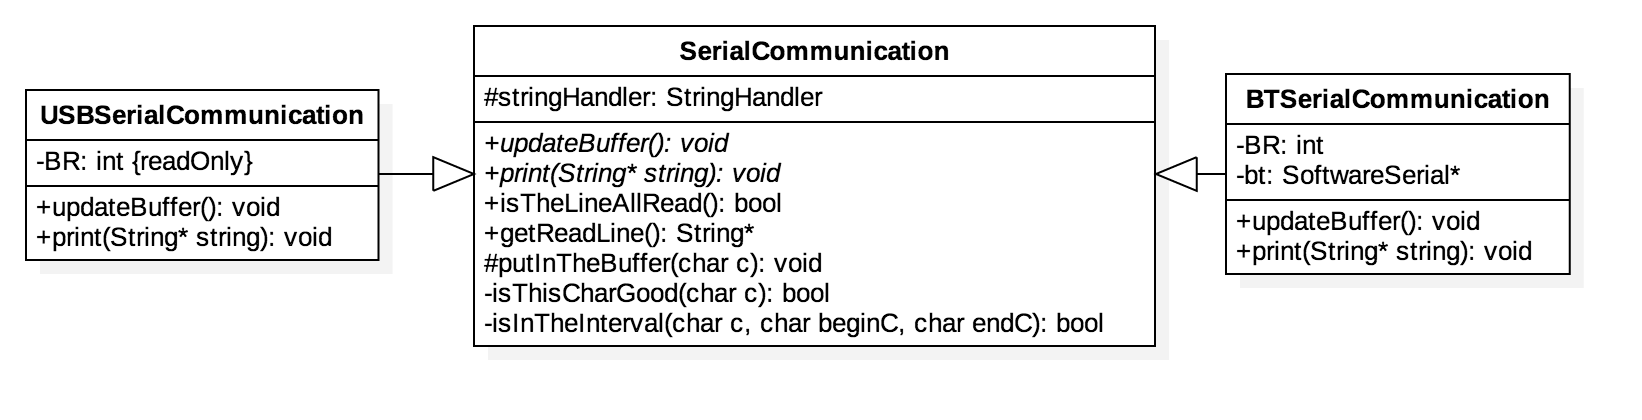
\includegraphics[width= 1.4\textwidth]
	{files/images/ArduinoConnection}
	\caption{The structure of the connection in the receiver.}
	\label{fig:connection}
\end{figure}
The \textit{SerialCommunication} can be seen as a temporary buffer where the character are provisionally stored until an end line token is received. For this reason this object provides few important method useful to this process:
\begin{itemize}
	\item \textit{updateBuffer}: this method is used to move the available characters from the receiver buffer to this object one. If there is no character or a line is fully read, this method simply does nothing.
	\item \textit{isAllTheLineRead} and \textit{readLine}: these methods are used to know if a line is fully read and, in positive case, converting all the read characters in a string, emptying the buffer.
	\item \textit{print}: this method is basically used to print something on the connection channel.
\end{itemize}
All the received characters are temporary stored in an apposite data structure, called \textit{StringHandler}. This encapsulates all the related methods, like the insertion and the string casting.\\*
In the Figure \ref{fig:connection}, in particular in the parent class, two methods are indicate as virtual, since their implementation depends by the connection type used. Consequently, the \textit{SerialCommunication} class was extended by \textit{BTSerialCommunication} and by \textit{USBSerialCommunication}, which implement these two methods, according to their specification and using proper attributes to perform these actions.\\*
In the communication, the class \textit{USBSerialCommunication} and the \textit{print} method of \textit{BTSerialCommunication} are implemented but never used. They were implemented for debug features and for future expansion, made easier by this organization.

\subsection{The Executer}
This object allows to interpret the received commands. A command is a string that has, as first character, a proper name and, subsequently, some parameters for that specific command. Its name is used to get, with a constant time through an Hash map, the method to invoke to execute that specific command. This structure allows to extends the robot with future module, without changing this object but just adding the new function pointers to the map.\\*
For instance, this robot uses the following commands:
???
\newpage

\subsection{The circuit}
\begin{figure}[h!]
	\centering
	\hspace*{-0.05 \textwidth}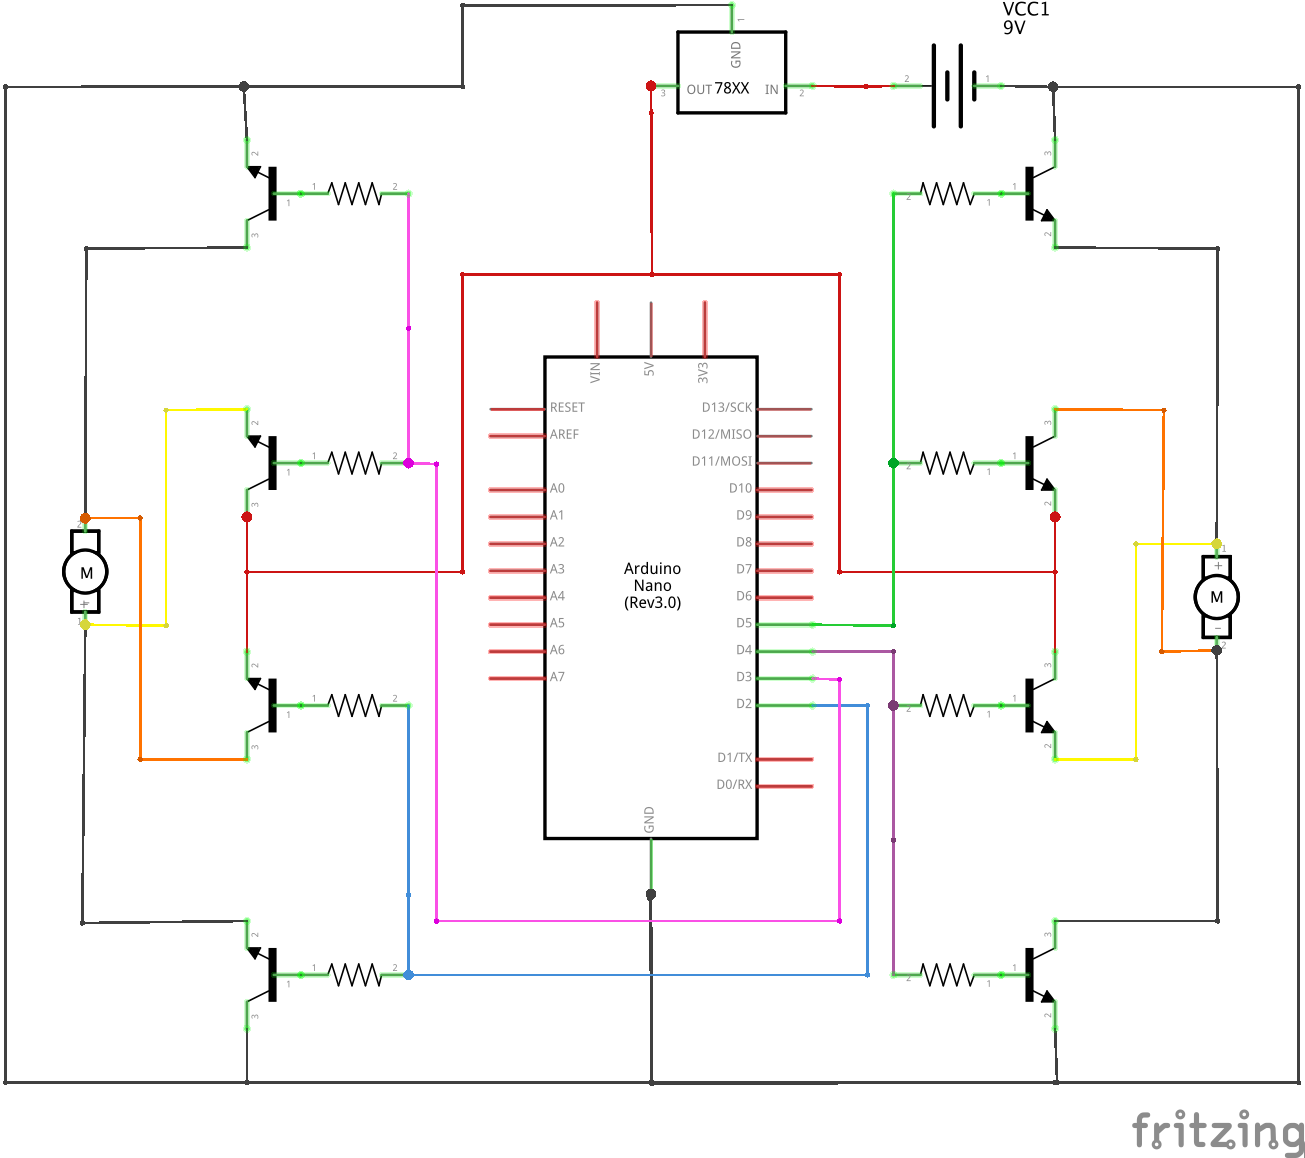
\includegraphics[width= 1.1\textwidth]
	{files/images/ReceiverScheme}
	\caption{The circuit scheme of the robot. The resistors are all of one KOhm.}
\end{figure}
This configuration uses eight BJTs to allow the motors to rotate in two different directions, allowing more moves for the robot. The voltage that they receive is around three volts.